\section{Diskussion}
\label{sec:Diskussion}

Die Versuchsdurchführung verlief ohne Probleme.
Die aufgenommenen Messwerte zeigen keine größeren Unregelmäßigkeiten.
Der verwendete Laser hat eine Wellenlänge von $\SI{635}{\nano\metre}$.
Aus den Messwerten heraus wurde eine Wellenlänge von $\SI{668.27 \pm 0.28}{\nano\metre}$ bestimmt.
Somit ergibt sich eine Abweichung von $(5.24 \pm 0.04) \%$.

\noindent
Bei der Bestimmung des Brechungsindexes für Luft wurde $n = 1.395 \pm 0.012$ ermittelt.
Im Vergleich zum Theoriewert von $1.00028$ \cite{brechungsindex} ergibt sich daraus eine Abweichung von $(28.3 \pm 0.6)\%$.
Diese Abweichung ist erheblich größer als die der Wellenlänge, aber kann durch einen Vorfall während der Versuchsdurchführung erklärt werden.
Durch das Evakuieren der Messzelle mithilfe der Vakuumpumpe gerieten die Schläuche, die die Pumpe und Messzelle verbinden, an die Schraube des justierbaren Spiegels.
Dadurch wurden kleine, aber merkliche Änderungen vorgenommen, sodass einige Versuchsgänge wiederholt wurden.

\section{Anhang}
\label{sec:Anhang}

\begin{figure}
    \centering
    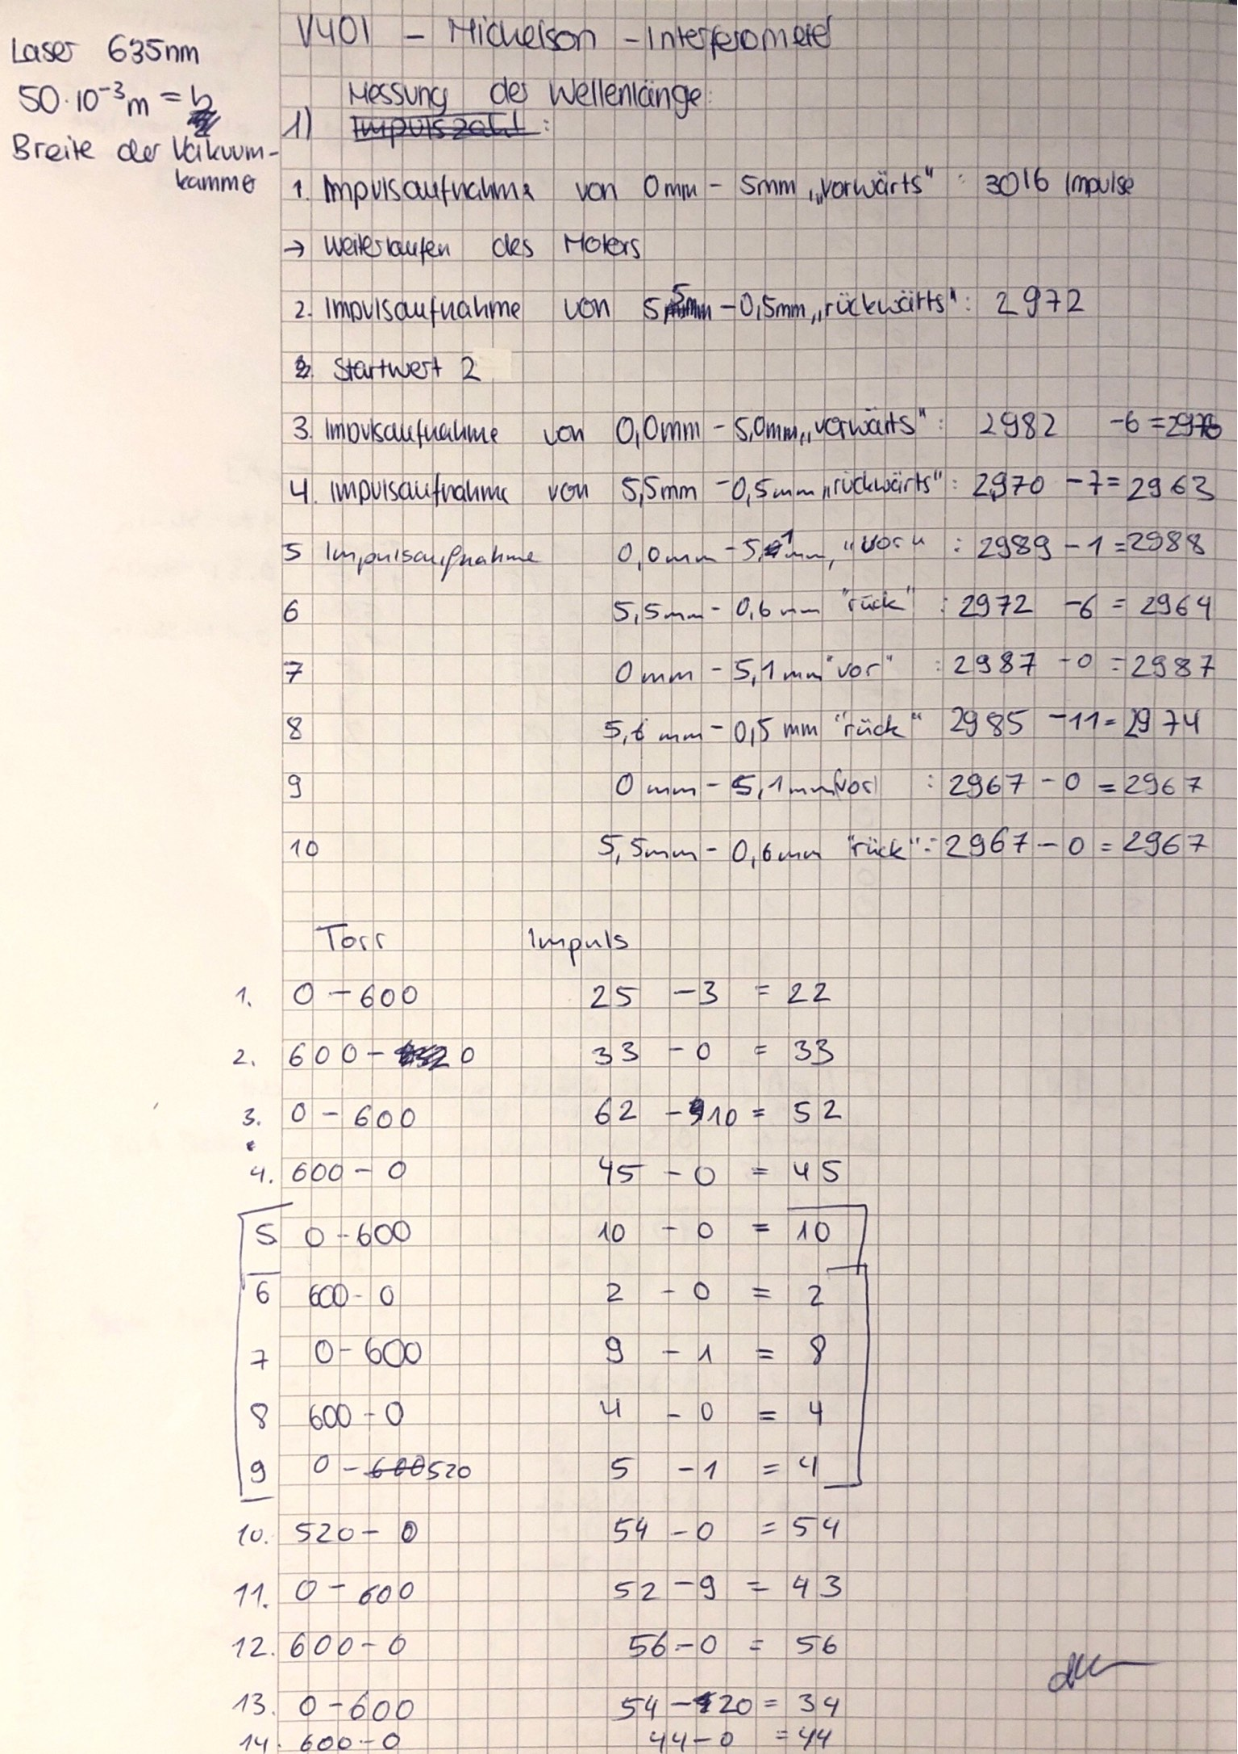
\includegraphics[width=\textwidth]{content/data_v401.pdf}
    \caption{Die notierten Werte von der Versuchsdurchführung.}
    \label{fig:datenmessung}
\end{figure}
